\documentclass[12pt, openright, a4paper, brazil, openany, oneside]{abntex2}

\usepackage{times}		
\usepackage[T1]{fontenc}	
\usepackage[utf8]{inputenc}	
\usepackage{indentfirst}	
\usepackage{color}			
\usepackage{graphicx}		
\usepackage{microtype} 		
\usepackage{multicol}
\usepackage{multirow}
\usepackage{lipsum}				
\usepackage[brazilian,hyperpageref]{backref}

\newtheorem{teo}{Teorema}
	 
\usepackage[alf]{abntex2cite}
\renewcommand{\backrefpagesname}{Citado na(s) página(s):~}
\renewcommand{\backref}{}
\renewcommand*{\backrefalt}[4]{
	\ifcase #1 %
		Nenhuma citação no texto.%
	\or
		Citado na página #2.%
	\else
		Citado #1 vezes nas páginas #2.%
	\fi}%
\titulo{Uma bissetriz paralela aplicada na construção triangular}
\autor{Sérgio Luís Soares Almeida \\ Matrícula 18/0006410}
\local{Brasília}
\data{14 de Novembro de 2018}
\instituicao{%
  Universidade de Brasília -- UnB
  \par
  Departamento de Matemática
  \par
 PROFMAT}
\tipotrabalho{Estudo de Artigo}

\definecolor{black}{RGB}{0.0,0.0,0.0}


\makeatletter

\preambulo{Estudo do artigo An Angle Bisector Parallel Applied to
Triangle Construction publicado em 13 de julho de 2009 disponível no endereço http://forumgeom.fau.edu/FG2009volume9/FG200915.pdf}

\hypersetup{pdftitle={\@title}, pdfauthor={\@author}, pdfsubject={\imprimirpreambulo}, pdfcreator={LaTeX with abnTeX2}, pdfkeywords={abnt}{latex}{abntex}{abntex2}{relatório técnico}, colorlinks=true, linkcolor=black, citecolor=black, filecolor=black, urlcolor=black, bookmarksdepth=4}
\makeatother

\setlength{\parindent}{1.3cm}


\setlength{\parskip}{0.2cm}  


\makeindex

\begin{document}


\selectlanguage{brazil}


\frenchspacing 


\imprimircapa

\imprimirfolhaderosto*

\ABNTEXchapterfont

\pdfbookmark[0]{\contentsname}{toc}
\tableofcontents*
\cleardoublepage
\textual

\chapter*[Introdução]{Introdução}
\addcontentsline{toc}{chapter}{Introdução}


Neste estudo construiremos o círculo de nove pontos, pois através de um deles (Ponto de Euler) provaremos um teorema que descreve uma linha paralela a uma bissetriz de um triângulo e passando pelo ponto médio do lado oposto. Nós então aplicaremos este teorema para a solução de quatro problemas de construção de triângulo.

% \let\clearpage\relax


\chapter{Pontos de Euler}

Neste capítulo iremos construir o círculo de nove pontos encontrados em um triângulo qualquer. O círculo de nove pontos é o círculo que contém os pontos médios, os pés das alturas e os pontos médios dos segmentos compreendidos entre o ortocentro e os vértices do triângulo, sendo esses últimos chamados de pontos de Euler.

Para esta construção iremos usar as seguintes notações:

\begin{itemize}
\item $\triangle ABC$ é o triângulo cujos vértices são, respectivamente $A$, $B$, e $C$.
\item O segmento $BC$ será o lado $a$, o segmento $AC$ será o lado $b$ e o segmento $AB$ será o lado $c$.

\begin{figure}[h]

    \center

    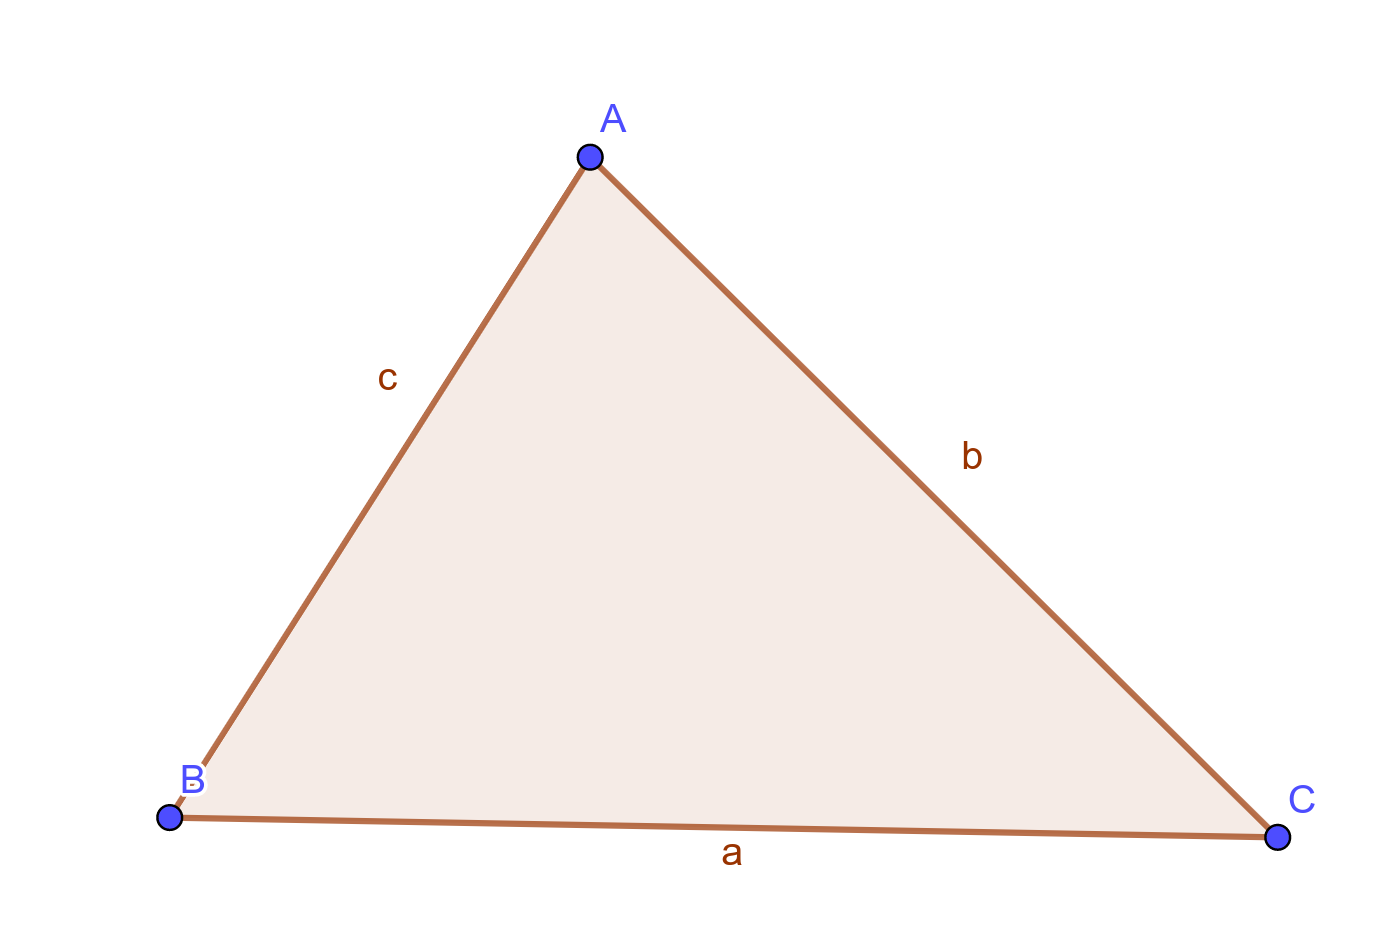
\includegraphics[width=8cm]{triangulo1.png}
    \caption{Triângulo \label{tria1}}
    
\end{figure}

\item $D$, $E$, e $F$ são os pés das alturas relativas aos lados $a$, $b$ e $c$ respectivamente.


\end{itemize} 


\section{Construindo o Círculo}

Considere o $\triangle ABC$ conforme a figura \ref{tria1} e nele traçamos as alturas relativas aos seus vértices, encontrando os pontos $D$, $E$, e $F$. Esses pontos são chamados de pés das alturas relativas.

\newpage

Considere agora o triângulo $\triangle DEF$ conforme a figura \ref{tria2} 

\begin{figure}[h]

    \center

    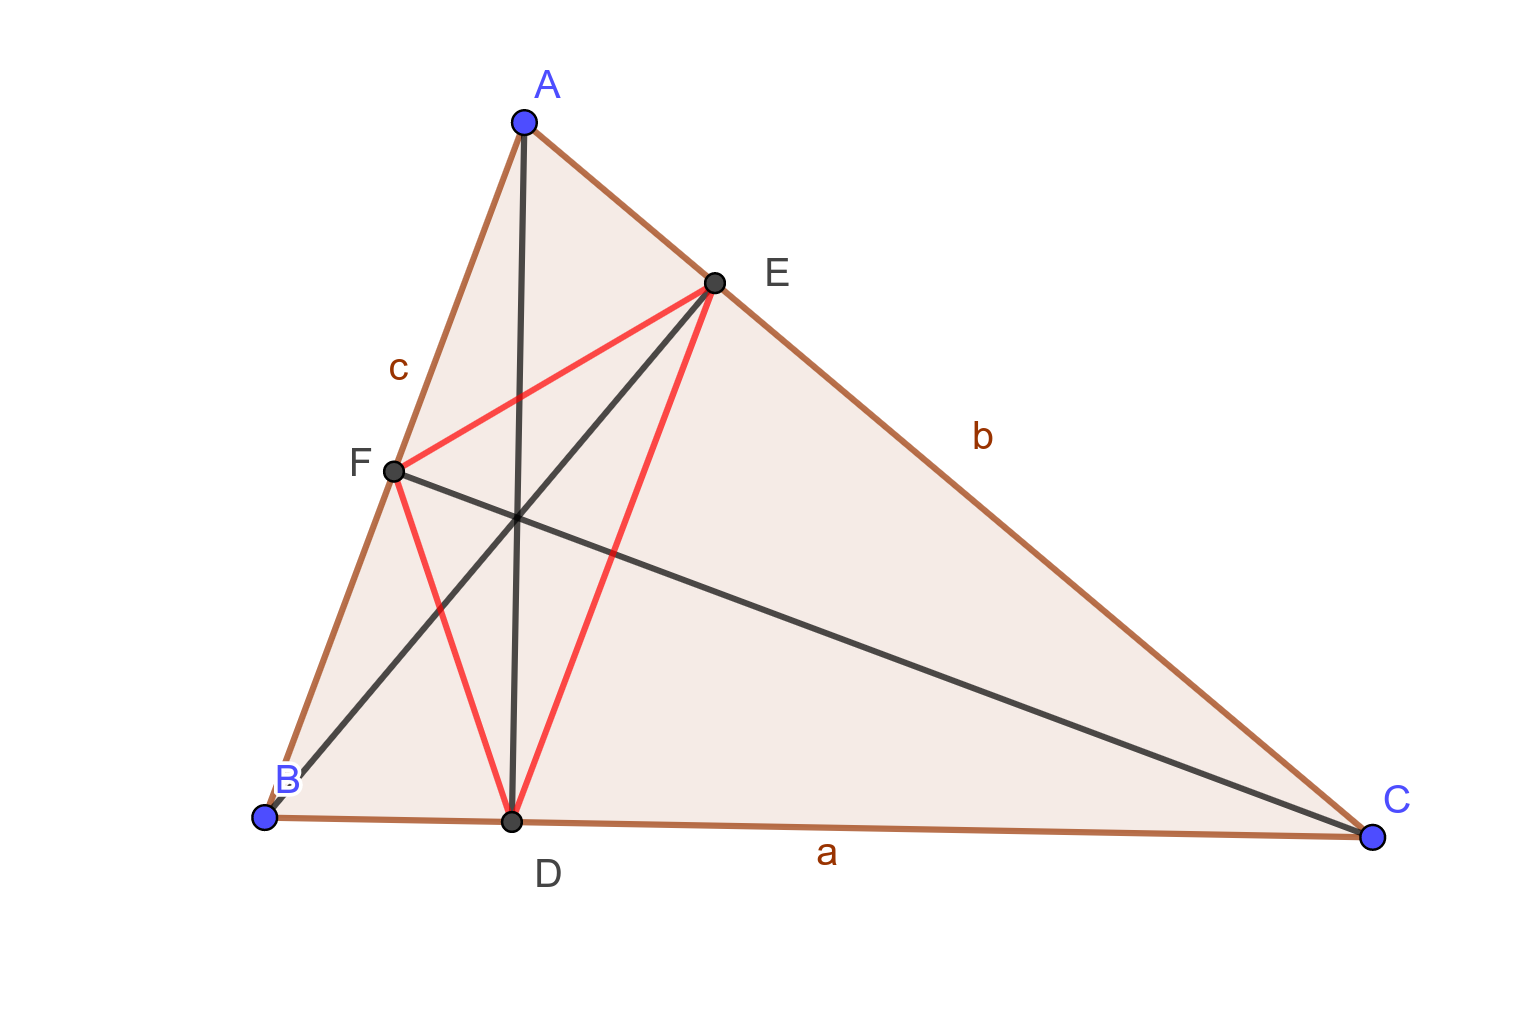
\includegraphics[width=6.9cm]{triangulo2.png}
    \caption{Alturas relativas e $\triangle DEF$ \label{tria2}}
    
\end{figure}

Vamos construir o círculo circunscrito neste triângulo e, para isso, devemos encontrar o seu circuncentro, pois este será o centro desse círculo.

Tracemos as mediatrizes referentes aos segmentos $DE$ e $EF$. O ponto de intersecção desses segmentos será o circuncentro e o raio do círculo circunscrito será a distância desse ponto a qualquer dos vértices do $\triangle DEF$.

\begin{figure}[h]

    \center

    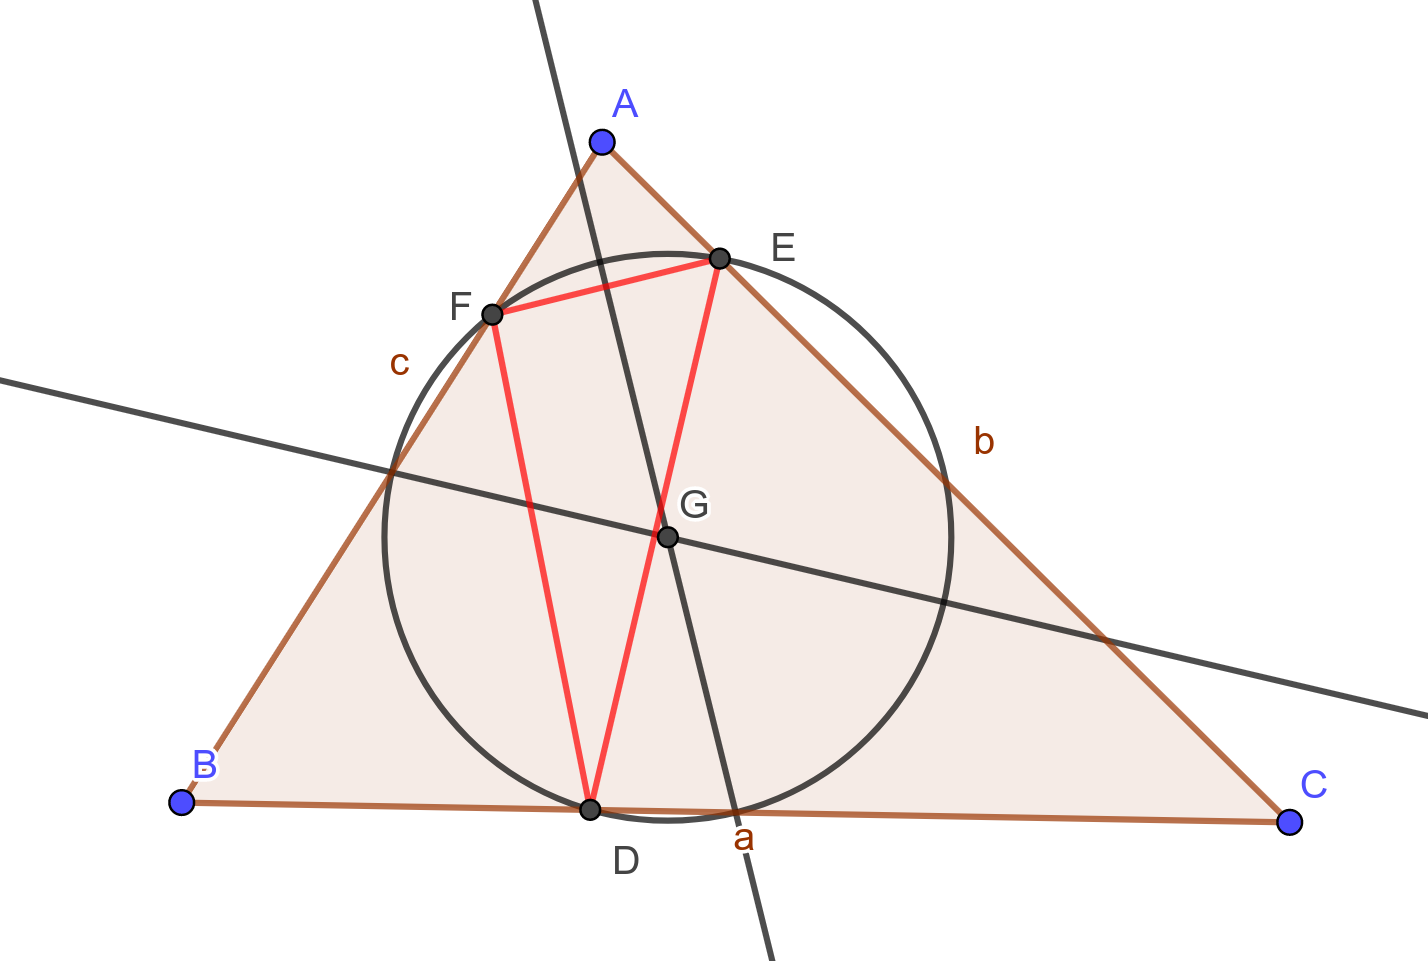
\includegraphics[width=6.9cm]{triangulo3.png}
    \caption{Alturas relativas e $\triangle DEF$ \label{tria3}}
    
\end{figure}

Este círculo terá 6 pontos de intersecção com o $\triangle ABC$: $D$, $E$, $F$, $H$, $I$ e $J$ e mais três pontos de intersecção com as alturas relativas aos lados desse triângulo: $K$, $L$ e $M$. Esses últimos três pontos são chamados de \textit{pontos de Euler}.

\begin{figure}[h]

    \center

    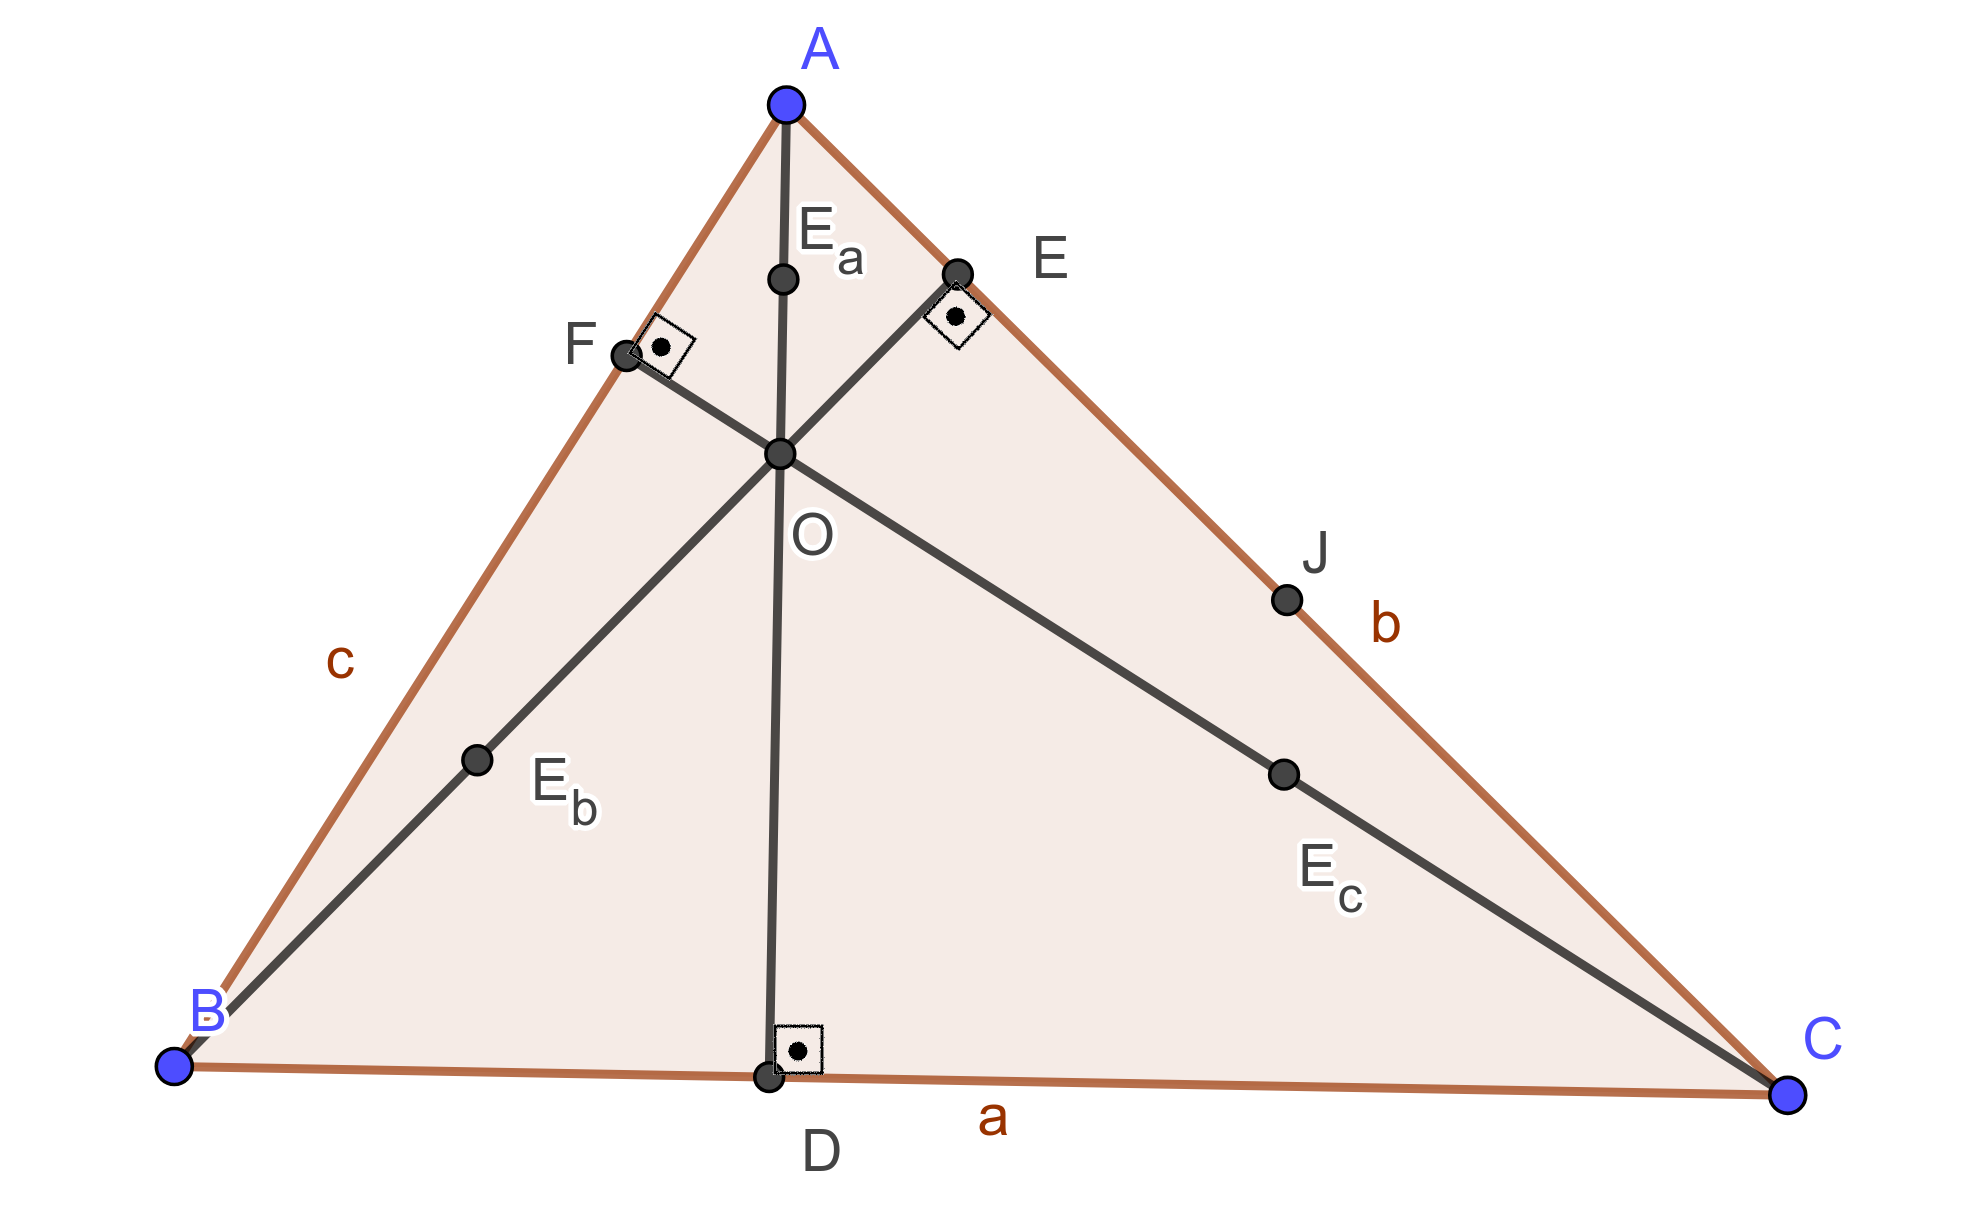
\includegraphics[width=6.9cm]{triangulo4.png}
    \caption{Alturas relativas e $\triangle DEF$ \label{tria4}}
    
\end{figure}

\chapter{O teorema da bissetriz e sua paralela}

Considere o triângulo $\triangle ABC$, com a bissetriz $AT_a$, altura $AH_a$, ponto médio $M_a$ relativo ao lado $BC$ e o ponto de Euler $E_a$, conforme figura ??? . Faça um círculo de centro $E_a$ passando por $M_a$ de tal forma que intercepte a reta suporte de $AH_a$ no ponto $P$. Trace a linha $M_{a}P$.

\begin{teo}\label{teo1}
	Em qualquer triângulo $\triangle ABC$ com $H_a$ não coincidindo com $M_a$, o segmento $M_{a}P$ é paralelo a bissetriz $AT_a$
\end{teo}


\begin{comment}
\chapter{Objetivos}

\begin{itemize}
    \item Aprender a diferença entre alguns sistemas de numeração
    \item Transformar, através da calculadora, números do sistema decimal para outros  sistemas, como o binário e o hexadecimal e vice-versa.
\end{itemize}


\chapter{Público alvo}

Alunos do Ensino Médio

\vspace{1cm}

\chapter{Tempo estimado}

3 aulas de 50 minutos
\vspace{1cm}



\chapter{Roteiro da Aula}
% ---
\section{História dos sistemas de numeração}

Descrever um pouco da história dos números e seus sistemas de numeração, como o sistema de números romanos, até chegarmos ao sistema mais usado na atualidade, que é o sistema decimal. Com isso mostramos que o sistema decimal é um sistema chamado posicional, isto é, que o valor de um determinado símbolo depende de sua posição, e o sistema romano não é posicional.

Tempo: 25 minutos
\section{Encontrar restos de divisão}

Usando a calculadora, devemos encontrar os restos de divisão, usando vários dividendos e divisores naturais. Para isso uma das possibilidades é fazer a divisão na calculadora e depois fazer a multiplicação apenas da parte inteira do número encontrado com o divisor e ver qual a diferença, com isso mostramos que o resto será sempre menor que o divisor. Aos poucos vamos nos concentrando na divisão por 2 e por 16, pois essas são as bases dos números binários e hexadecimais.

Tempo: 25 minutos

\section{Transformar números decimais em binários}
Novamente usando a calculadora, transformaremos os números decimais em binários. Para isso dividimos uma lista de números naturais por 2 sucessivamente, anotando os restos dessa divisão. Mostramos que a leitura desses restos na ordem inversa é o número transformado em binário. Por exemplo, transformar o número 45 em binário.

\begin{figure}[h]

    \center

%    \includegraphics[width=7cm]{binariofim.png}

\end{figure}


Então usamos a tabela:

 \begin{table}[h]
        \centering
        \begin{tabular}{|c|c|c|c|}
            \hline
            Dividendo & Divisor & Quociente & Resto \\
            \hline
            45 & 2 & 22 & 1 \\
            \hline
            22 & 2 & 11 & 0 \\
            \hline
            11 & 2 & 5 & 1 \\
            \hline
            5 & 2 & 2 & 1 \\
            \hline
            2 & 2 & 1 & 0 \\
            \hline
            1 & 2 & 0 & 1 \\
            \hline
        \end{tabular}
    \end{table}
Assim, o número 45 escrito em binário é igual a 101101.

Usar outros exemplos de transformação de números naturais em binários.

Tempo: 30 minutos


\section{Transformar números naturais em hexadecimal (tabela ASCII)}

Um dos sistemas também muito usado é o sistema hexadecimal. Ele é usado muito na computação através da tabela ASCII. A transformação de um número decimal em hexadecimal usa uma correspondência entre restos de divisão e os algarismos e letras do alfabeto de acordo com a tabela abaixo:

\begin{table}[h]
        \centering
        \begin{tabular}{|l|c|c|c|c|c|c|c|c|c|c|c|c|c|c|c|c|}
            \hline
            Restos da divisão & 0 & 1 & 2 & 3 & 4 & 5 & 6 & 7 & 8 & 9 & 10 & 11 & 12 & 13 & 14 & 15 \\
            \hline
            Símbolo hexadecimal & 0 & 1 & 2 & 3 & 4 & 5 & 6 & 7 & 8 & 9 & A & B & C & D & E & F \\
            \hline
        \end{tabular}
    \end{table}

Exemplo: Usando a tabela acima, transformar o número decimal 23870 em número hexadecimal.

Da mesma forma como fazemos com o sistema binário, usamos a calculadora para fazer as divisões e encontrarmos os restos da divisão e preenchemos a tabela:

 \begin{table}[h]
        \centering
        \begin{tabular}{|c|c|c|c|}
            \hline
            Dividendo & Divisor & Quociente & Resto \\
            \hline
            23870 & 16 & 1491 & 14 \\
            \hline
            1491 & 16 & 93 & 3 \\
            \hline
            93 & 16 & 5 & 13 \\
            \hline
            5 & 16 & 0 & 5 \\
            \hline
        \end{tabular}
    \end{table}

Usando a tabela e lembrando que temos que ler na ordem inversa, o número hexadecimal é 5D3E.


É interessante também mostrar como os computadores usam esses números hexadecimais para relacioná-los com os caracteres do computador. Essa relação é feita através da tabela:

\begin{figure}[h]

    \center

%    \includegraphics[width=15cm]{tabelaascii.jpg}

\end{figure}


Tempo: 30 minutos



\section{Transformar números binários em números naturais}

Para transformarmos um número binário em número natural usaremos a fórmula $ V=S \cdot B^p $, onde:

\begin{itemize}
    \item V é o valor posicional do símbolo
    \item S é o valor absoluto do símbolo
    \item B é a base do sistema numérico
    \item P é a posição do símbolo em relação ao número, que é definida da direita para a esquerda e começa do zero.
\end{itemize}

Usaremos também a função memória da calculadora. Por exemplo, transformar o número binário 101101 em número natural.

\begin{table}[h]
        \centering
        \begin{tabular}{|l|c|c|c|c|c|c|}
            \hline
            Posição & 5 & 4 & 3 & 2 & 1 & 0 \\
            \hline
            Símbolo & 1 & 0 & 1 & 1 & 0 & 1 \\
            \hline
        \end{tabular}
    \end{table}


Assim, fazemos:

\begin{itemize}
    \item $V=1 \cdot 2^5=32 $ para a posição 5: e guardamos na memória da calculadora
    \item $V=0 \cdot 2^4=0 $ para a posiçao 4: e guardamos na memória da calculadora
    \item $V=1 \cdot 2^3=8 $ para a posição 3: e guardamos na memória da calculadora
    \item $V=1 \cdot 2^2=4 $ para a posição 2: e guardamos na memória da calculadora
    \item $V=0 \cdot 2^1=0 $ para a posição 1: e guardamos na memória da calculadora
    \item $V=1 \cdot 2^0=1 $ para a posição 0: e guardamos na memória da calculadora
\end{itemize}

Ao ler a memória da calculadora encontramos o resultado: 45.
Podemos também fazer a conversão de símbolos da tabela hexadecimal para números naturais da mesma forma.

Tempo: 40 minutos



\chapter{Considerações finais}

O uso da calculadora em sala de aula é um ótimo atrativo para os alunos, que não precisarão usar o tempo em cálculos repetitivos, o professor ainda pode aproveitar essa aula para estender os conhecimentos de sistema de numeração e comentar como funciona as definições de k (Kilo), M (Mega) e G (Giga), tanto para computadores, como para outros sistemas de numeração, pois essas formas de escrita de números aparecem com mais frequência hoje em dia, mas o professor deve sempre se lembrar que a calculadora não irá sempre resolver os problemas de sistemas de numeração, pois como foi colocado no planejamento, um exemplo de sistema de numeração como os romanos não é posicional e, portanto, a calculadora não irá ajudar muito. 




\end{comment}
\end{document}
